\chapter{Additional Photos}
\begin{figure}[h]
    \centering
    \begin{subfigure}{0.49\linewidth}
        \rotatebox{270}{\includegraphics[width=\linewidth]{Thesis/appendix/photos/dramatic-1.jpg}}
    \end{subfigure}
    \hfill
    \begin{subfigure}{0.49\linewidth}
        \rotatebox{270}{\includegraphics[width=\linewidth]{Thesis/appendix/photos/dramatic-2.jpg}}
    \end{subfigure}
    \begin{subfigure}{0.49\linewidth}
        \rotatebox{270}{\includegraphics[width=\linewidth]{Thesis/appendix/photos/dramatic-3.jpg}}
    \end{subfigure}
    \caption{Photos of model with dark background.}
    \label{fig:dramatic}
\end{figure}

\begin{figure}[h]
\begin{subfigure}[b]{0.475\textwidth}
            \centering
            \rotatebox{270}{\includegraphics[width=\textwidth]{Thesis/appendix/photos/right-view.jpg}}
            \caption[]%
            {{\small Right View}}    
            \label{fig:right-view}
        \end{subfigure}
        \hfill
        \begin{subfigure}[b]{0.475\textwidth}  
            \centering 
            \rotatebox{270}{\includegraphics[width=\textwidth]{Thesis/appendix/photos/left-view.jpg}}
            \caption[]%
            {{\small Left View}}    
            \label{fig:left-view}
        \end{subfigure}
        \vskip\baselineskip
        \begin{subfigure}[b]{0.475\textwidth}   
            \centering 
            \rotatebox{270}{\includegraphics[width=\textwidth]{Thesis/appendix/photos/back-view.jpg}}
            \caption[]%
            {{\small Back View}}    
            \label{fig:back-view}
        \end{subfigure}
        \hfill
        \begin{subfigure}[b]{0.475\textwidth}   
            \centering 
            \rotatebox{270}{\includegraphics[width=\textwidth]{Thesis/appendix/photos/top-view.jpg}}
            \caption[]%
            {{\small Top View}}    
            \label{fig:Top View}
        \end{subfigure}
\caption{Various angles of the robot.}
\label{fig:angle-pics}
\end{figure}

\begin{figure}[h]
    \centering
    \begin{subfigure}{0.49\linewidth}
        \centering
        \includegraphics[width=\linewidth,angle=270]{Thesis/appendix/photos/innerds-eye.jpg}
        \caption{}
    \end{subfigure}\hfill
    \begin{subfigure}{0.49\linewidth}
        \centering
        \includegraphics[width=\linewidth]{Thesis/appendix/photos/innerds-top.jpg}
        \caption{}
    \end{subfigure}
    \caption{Additional photos of the inner workings inside the head.}
    \label{fig:inner-workings}
\end{figure}

\begin{figure}[h]
    \centering
    \begin{subfigure}{0.35\linewidth}
        \centering
        \includegraphics[width=\textwidth,angle=270]{Thesis/appendix/photos/skeleton.jpg}
        \caption{Core Skeleton.}
    \end{subfigure}
    \begin{subfigure}[b]{0.25\linewidth}
        \centering
        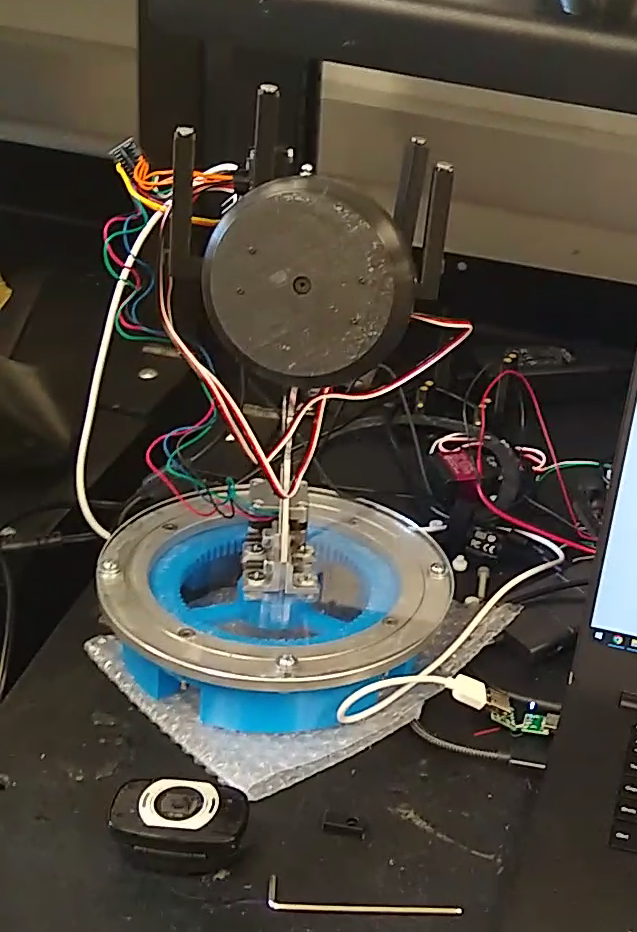
\includegraphics[width=\textwidth]{Thesis/appendix/photos/bare-robot.png}
        \caption{Head plates removed.}
    \end{subfigure}
    \begin{subfigure}{0.35\linewidth}
        \centering
        \includegraphics[width=\textwidth,angle=270]{Thesis/appendix/photos/before-painting.jpg}
        \caption{Before painting.}
    \end{subfigure}
    \caption{Various photos of the intermediary steps in making the robot.}
    \label{fig:my_label}
\end{figure}